\documentclass[aspectratio=43]{beamer}

\usepackage[utf8]{inputenc}

\usepackage{color}
\usepackage{listings}
\usepackage{tikz}
\usepackage{hyperref}

\usetheme{Rochester}
\usecolortheme{beaver}

\addtobeamertemplate{navigation symbols}{}{%
    \usebeamerfont{footline}%
    \usebeamercolor[fg]{footline}%
    \hspace{1em}%
    \insertframenumber/\inserttotalframenumber
}

\lstloadlanguages{C++}
    \lstset{%
        language={C++},
        basicstyle=\ttfamily,
        keywordstyle=\color{blue},
        showstringspaces=false,
        escapechar={§},
        escapeinside=||
    }

\newif\iftransitions
 \transitionstrue


\newif\iffast
% \fasttrue

\title{Why are rvalues \texttt{const}?}
%\subtitle{Lua for C++ Programmers}
\author{Andreas Weis}
\institute{BMW AG}
\date{MUC++, December 19, 2017}
%\titlegraphic{
\includegraphics[height=.25\textheight]{resources/cppcon.png}}


\begin{document}

\frame{\titlepage}

\iffalse
\begin{frame}[fragile]
  \frametitle{lvalues and rvalues}

  \begin{center}
  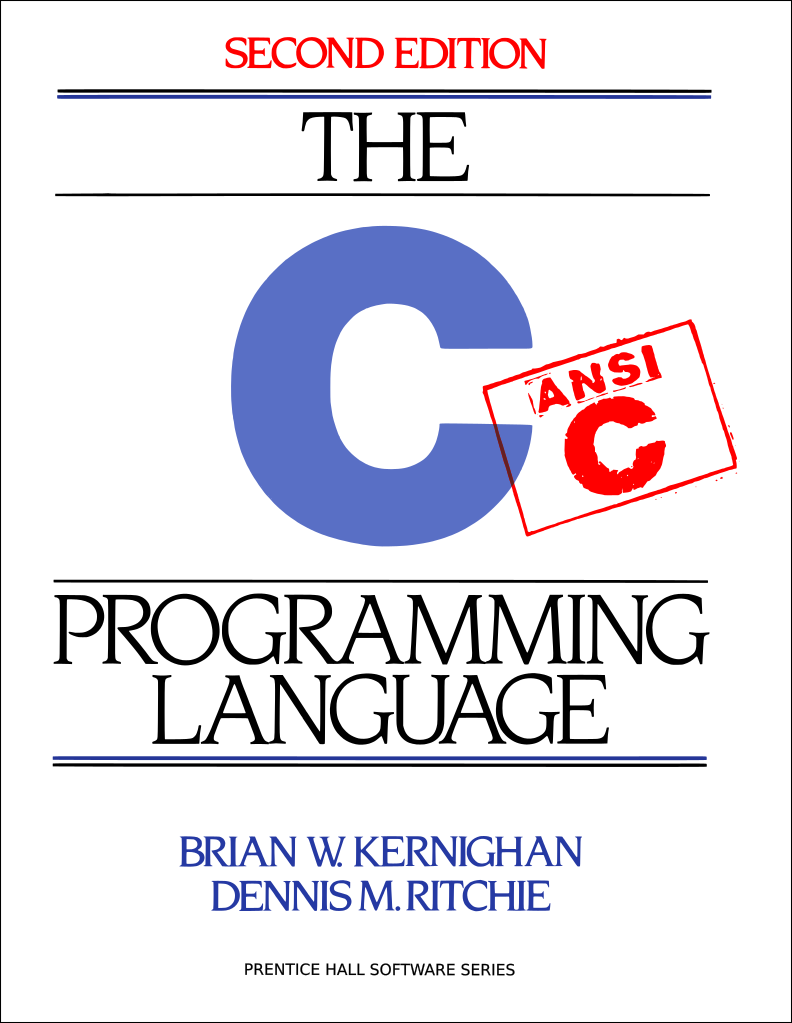
\includegraphics[height=.45\textheight]{resources/kr_tcpl.png}
  \end{center}

  \begin{quote}
  An \emph{object} is a named region of storage; an \emph{lvalue} is an expression referring to an object.
  [...]
  
  The name "lvalue" comes from the assignment expression \texttt{E1 = E2} in which the left operand \texttt{E1} must be an lvalue expression.
  \end{quote}
\end{frame}
\fi

\begin{frame}[fragile]
  \frametitle{Spot the bug!}
  \pause
  \begin{semiverbatim}
{\color{blue}struct} X \{
    {\color{blue}int} foo;
\};

{\color{blue}void} printX(X\& x) \{
    std::cout << x.foo << '\\n';
\}

X createX() \{ {\color{gray}\emph{/* ... */}} \}

{\color{blue}int} main()
\{
    printX(createX());
\}
  \end{semiverbatim}
\end{frame}


\begin{frame}[fragile]
  \frametitle{Spot the bug!}
  \begin{semiverbatim}
{\color{blue}struct} X \{
    {\color{blue}int} foo;
\};

{\color{blue}void} printX(X {\color{red}const}\& x) \{
    std::cout << x.foo << '\\n';
\}

X createX() \{ {\color{gray}\emph{/* ... */}} \}

{\color{blue}int} main()
\{
    printX(createX());
\}
  \end{semiverbatim}
\end{frame}


\begin{frame}
  \frametitle{But in order to understand...}
  \pause
  \begin{center}
  
\includegraphics[height=.85\textheight]{resources/btt80s.jpg}
  \end{center}
\end{frame}


\begin{frame}[fragile]
  \frametitle{Operator overloading}
  \begin{lstlisting}
int ix = 1;
int iy = 2;
int iz = ix + iy;
  \end{lstlisting}
  \pause
  \begin{lstlisting}
complex cx(1, 0);
complex cy(2, 0);
complex cz = cx + cy;
  \end{lstlisting}
\end{frame}

\begin{frame}[fragile]
  \frametitle{Operator overloading (by-value)}
  \begin{lstlisting}
complex operator+(complex x, complex y)
{
    return complex(x.real() + y.real(),
                   x.imag() + y.imag());
}

complex cz = cx + cy;
  \end{lstlisting}
\end{frame}


\begin{frame}[fragile]
  \frametitle{Operator overloading (by-pointer)}
  \begin{lstlisting}
complex operator+(complex* x, complex* y)
{
    return complex(x->real() + y->real(),
                   x->imag() + y->imag());
}

complex cz = &cx + &cy;     // ???
  \end{lstlisting}
\end{frame}


\begin{frame}[fragile]
  \frametitle{Operator overloading (by-pointer)}

  \begin{lstlisting}
auto      foo = &cx - &cy;       // ??????
  \end{lstlisting}
\end{frame}

\begin{frame}[fragile]
  \frametitle{Operator overloading (by-pointer)}

  \begin{lstlisting}
ptrdiff_t foo = &cx - &cy;       // !
  \end{lstlisting}
\end{frame}


\begin{frame}[fragile]
  \frametitle{Operator overloading}
  \pause
  \begin{lstlisting}
complex operator+(complex& x, complex& y)
{
    return complex(x.real() + y.real(),
                   x.imag() + y.imag());
}

complex cz = cx + cy;
  \end{lstlisting}
\end{frame}


\begin{frame}[fragile]
  \frametitle{References - syntactic ambiguities}

  \begin{lstlisting}
    complex* px = &cx;
    complex* py = &cy;

    px  = py;
    *px = *py;
  \end{lstlisting}
  \pause
  \begin{lstlisting}
    complex& rx = cx;
    complex& ry = cy;

    rx = ry;        // ???
  \end{lstlisting}
\end{frame}

\begin{frame}[fragile]
  \frametitle{References}
References cannot be re-bound. \vspace{.1\textheight}

A \texttt{T\&} behaves like a \texttt{T* const}.
\end{frame}


\begin{frame}[fragile]
  \frametitle{The end.}

  \pause
  \begin{center}
  
\includegraphics[height=.85\textheight]{resources/biff.jpg}
  \end{center}
\end{frame}


\begin{frame}[fragile]
  \frametitle{Just one more thing...}
  
  \begin{lstlisting}
  void incr(int& ri) { ri++; }

  void g()
  {
      long l = 1;
      incr(l);
  }
  \end{lstlisting}
\end{frame}


\begin{frame}
  \frametitle{If you want to know more...}

  \begin{center}
  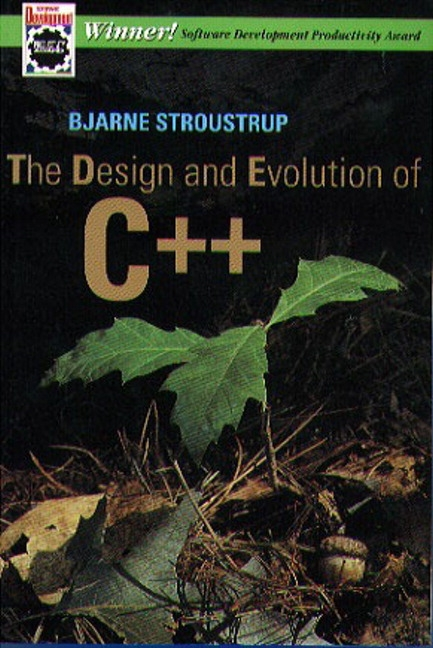
\includegraphics[height=.45\textheight]{resources/de_cpp.jpg}
  \end{center}
  
  \begin{itemize}
    \item The Design and Evolution of C++ (Addison-Wesley, 1994)
    \item \href{http://www.stroustrup.com/hopl2.pdf}{A History of C++: 1979 - 1991 (HOPL-II, 1993)}
    \item \href{http://www.stroustrup.com/hopl-almost-final.pdf}{Evolving a language in and for the real world: C++ 1991-2006 (HOPL-III, 2007)}
  \end{itemize}


\end{frame}

\begin{frame}
  \frametitle{Thanks for your attention.}
\end{frame}


\end{document}
